\documentclass[12pt,a4paper]{report}

\usepackage{fontspec}
\setmainfont{Times New Roman}
\usepackage[top=3cm, bottom=3cm, left=4cm, right=3cm]{geometry}

\usepackage{indentfirst}
\usepackage{graphicx}
\usepackage{setspace}
\usepackage{fancyhdr}
\setlength{\headheight}{15pt}

% --- Nomor halaman di KANAN ATAS ---
\fancypagestyle{skripsi}{
  \fancyhf{}
  \fancyhead[R]{\thepage}
  \renewcommand{\headrulewidth}{0pt}
  \renewcommand{\footrulewidth}{0pt}
}

% --- Penomoran seperti dokumen utama (BAB IV -> Tabel 4.x, Gambar 4.x) ---
\renewcommand{\thesection}{\arabic{chapter}.\arabic{section}}
\renewcommand{\thetable}{\arabic{chapter}.\arabic{table}}
\renewcommand{\thefigure}{4.92}
\renewcommand{\figurename}{Gambar}
\renewcommand{\tablename}{Tabel}

\setlength{\parindent}{1.27cm}
\setlength{\parskip}{12pt}

% --- Format sub-bab ---
\usepackage{titlesec}
\titleformat{\section}{\normalfont\bfseries}{\thesection}{1em}{}
\titlespacing*{\section}{0pt}{2pt}{-6pt}
\titleformat{\subsection}{\normalfont\bfseries}{\thesubsection}{1em}{}
\titlespacing*{\subsection}{0pt}{2pt}{-6pt}

% --- Format caption gambar & tabel ---
\usepackage{caption}
\captionsetup[figure]{labelfont=bf, textfont=normalfont, labelsep=space, justification=centering}
\captionsetup[table]{labelfont=bf, textfont={normalfont, stretch=1}, labelsep=space, justification=raggedright, singlelinecheck=false, skip=0pt, margin=0pt, indention=0pt}

% --- Anti pemenggalan kata & widow/orphan ---
\tolerance=1
\emergencystretch=\maxdimen
\hyphenpenalty=10000
\hbadness=10000
\widowpenalty=10000
\clubpenalty=10000
\displaywidowpenalty=10000

% --- Gambar tetap di tempat (H) ---
\usepackage{float}
\floatplacement{figure}{H}

% --- Konfigurasi longtable (spasi 1, font 10pt) ---
\usepackage{longtable}
\usepackage{array}
\setlength{\LTcapwidth}{\textwidth}
\setlength{\extrarowheight}{3pt}
\AtBeginEnvironment{longtable}{\singlespacing\fontsize{10}{12}\selectfont}
\setlength{\LTpre}{0pt}
\setlength{\LTpost}{0pt}

\setcounter{secnumdepth}{3}

% --- Counter palsu supaya nomor sesuai dokumen utama ---
\setcounter{page}{145}
\setcounter{chapter}{4}
\setcounter{section}{2}
\setcounter{table}{4}

\begin{document}
\pagestyle{skripsi}
\setstretch{1.5}

\section{\emph{Lighthouse Testing}}

\emph{Lighthouse testing} dilakukan untuk mengukur kualitas aplikasi web secara keseluruhan, khususnya dalam memenuhi standar PWA. Pengujian ini mencakup 4 metrik utama: \emph{Performance}, \emph{Accessibility}, \emph{Best Practices}, dan SEO. Pengujian dilakukan pada halaman utama aplikasi (\emph{dashboard}) menggunakan \emph{DevTools Lighthouse} bawaan \emph{browser}. Ringkasan hasil pengujian dapat dilihat pada Tabel \ref{tab:pengujian-lighthouse} berikut.

\captionsetup[longtable]{justification=raggedright, singlelinecheck=false}
\setlength{\LTcapwidth}{11cm}
\addtolength{\LTcapwidth}{8\tabcolsep}
\addtolength{\LTcapwidth}{5\arrayrulewidth}
\begin{longtable}{|>{\centering\arraybackslash}p{1cm}|p{4.5cm}|>{\centering\arraybackslash}p{2.5cm}|>{\centering\arraybackslash}p{3cm}|}
\caption{Tabel Hasil \textit{Lighthouse Testing} } \label{tab:pengujian-lighthouse} \\
\hline
\textbf{No} & \textbf{Kategori Metrik} & \textbf{Skor} & \textbf{Status} \\ \hline
\endfirsthead \hline
\textbf{No} & \textbf{Kategori Metrik} & \textbf{Skor} & \textbf{Status} \\ \hline
\endhead \hline
\endfoot
1 & \textit{Performance} & 97 & Baik \\ \hline
2 & \textit{Accessibility} & 100 & Baik \\ \hline
3 & \textit{Best Practices} & 100 & Baik \\ \hline
4 & SEO & 100 & Baik \\ \hline
\end{longtable}

\begin{figure}[H]
\centering
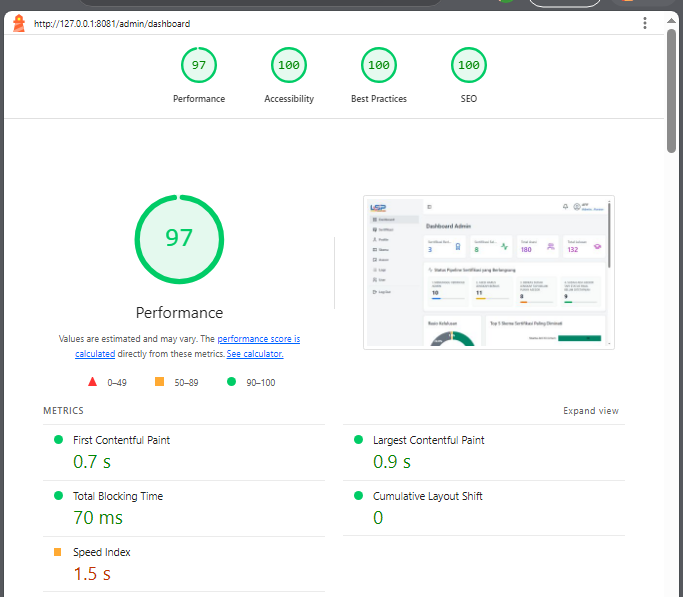
\includegraphics[width=\textwidth, keepaspectratio]{images/lighthouse-test.png}
\caption{Hasil \textit{Lighthouse testing} \label{fig:lighthouse-test}}
\end{figure}

\end{document}
